\documentclass{article}
\author{Giulio Incoronato, Antonio Mazzarella}
\usepackage{graphicx}
\usepackage{fancyhdr}
\usepackage{hyperref}
\usepackage{lipsum} %for some dummy text
\usepackage{array} %per gli array in tabella
\usepackage[table]{xcolor} %colori della tabella
\newcommand{\mytextbf}[1]{\textbf{\bfseries #1}}
\usepackage{tabularx}
\usepackage{geometry}
\usepackage{pgf-pie}

%variabili globali
\newcommand{\mainname}{UGotTheJob}


\geometry{
    a4paper,
    total={170mm,257mm},
    left=20mm,
    top=20mm,
}


%di seguito imposterò i piè pagina
\pagestyle{fancy}
\fancyhf{}
\fancyfoot[L]{\thepage}
\fancyfoot[R]{\includegraphics[height=40pt]{job_seeking.png}}
\setlength{\footskip}{43.60004pt}

%font utilizzato san serif
\renewcommand{\headrulewidth}{0pt} % rimuovi la linea dell'header
\renewcommand{\familydefault}{\sfdefault}

\begin{document}
\thispagestyle{empty}

\begin{center}%inizio documento
    \includegraphics[scale=0.6]{job_seeking.png}

    \vspace{1cm}

    \textbf{\huge{\mainname}} % Aggiunge il titolo

    \vspace{0.5cm}

    \fontsize{17}{16}
    \textbf{Artificial Intelligence DOCUMENT}

    \textit{"Dipartimento di Informatica anno 2022/2023"}

    \textit{"Professore: Fabio Palomba"}

    \vspace{1.8cm}


    \begin{table}[ht]
        \fontsize{17}{12}\selectfont
        \centering
        \setlength{\arrayrulewidth}{2pt}
        \setlength{\tabcolsep}{5pt}
        \def\arraystretch{1.8}
        \begin{tabular}{ c | c }
            \textbf{Autori}    & \textbf{Matricola} \\
            \hline
            Giulio Incoronato  & 0512111363         \\
            Antonio Mazzarella & 0512112830         \\
        \end{tabular}
    \end{table}
\end{center}

\newpage %nuova pagina

\tableofcontents

\newpage

\section{Introduzione}
Quante volte hai avuto l'ansia di essere preso o pure no in uno specifico lavoro?
Quante volte ti sei domandato se fossi giusto tu per quel lavoro? Con la fine del proprio percorso
di studio ci si pongono tante domande e dubbi se si viene presi in un determinato lavoro oppure no.
\par
Tutto questo sorge perchè dopo diversi anni di studio si vuole avere la sicurezza di essere presi
in un determinato lavoro, magari il lavoro dei propri sogni. Sarebbe utile avere un tool in grado di
prevedere, attraverso dei dati, se sarai preso.
\par
Il nostro team mira a combattere tutte queste ansie creando un tool chiamato \textbf{"\mainname"}
che integrerà algoritmi di machine learning supervisionato che andranno ad analizzare un dataset
in modo da prevedere i risultati in base agli input forniti dall'utente.

\subsection{Link Utili}
\begin{enumerate}
    \item Questo è il link alla repository ufficiale di \textbf{\mainname}: \href{https://github.com/ShackWove/GuessUJob}{Link}
    \item Questo è il link dove abbiamo preso i dataset usati per l'addestramento: \href{https://www.kaggle.com/datasets/ahsan81/job-placement-dataset}{Link}
    \item Qui è dove è stata presa l'immagine: \href{https://www.flaticon.com/free-icon/job-seeking_1503438}{Link}
\end{enumerate}

\section{Specifiche P.E.A.S.}

\begin{table}[ht]
    \centering
    \rowcolors{1}{gray!5}{gray!15}
    \begin{tabular}{| l | m{8cm} |}
        \hline
        \textbf{Performance} & Capacità dell'agente di prevedere se l'utente sarà preso o meno per un lavoro.                       \\
        \textbf{Enviroment}  & L'ambiente in cui l'agente opera rappresentato da un form di cui l'utente scriverà i dati necessari. \\
        \textbf{Actuators}   & Interfaccia utente dell'applicazione dove uscirà il valore predetto.                                 \\
        \textbf{Sensors}     & Form nell'interfaccia utente.                                                                        \\
        \hline
    \end{tabular}
\end{table}
\subsection{Proprietà dell'Ambiente}
L'ambiente possiede le seguenti proprietà:
\begin{itemize}
    \item \textbf{Completamente osservabile:} l'agente ha accesso completo a tutte le informazioni fornite dall'utente.
    \item \textbf{Deterministico:} lo stato dell'ambiente dipende dall'azione intrapresa dall'agente.
    \item \textbf{Sequenziale:} le decisioni dell'agente dipendono dagli input dell'utente.
    \item \textbf{Statico:} nel momento in cui l'agente sta elaborando la sua previsione l'utente non può modificare il form dato in partenza.
    \item \textbf{Discreto:} le previsioni dell'agente dipendono soprattutto dagli input inseriti dall'utente, oltretutto c'è un numero limitato e preciso di informazioni che l'utente può inserire.
    \item \textbf{Singolo-agente:} esiste solo un agente che opera nell'ambiente.
\end{itemize}

\newpage

\section{Machine Learning}
Il machine learning (apprendimento automatico) è una tecnologia dell'intelligenza artificiale che consente alle macchine di imparare dai dati, senza essere esplicitamente programmate. In altre parole, il machine learning si basa sulla costruzione di algoritmi che possono imparare da un insieme di dati e migliorare la loro capacità di risolvere compiti specifici con l'esperienza.

Ci sono tre tipi principali di apprendimento automatico:
\begin{itemize}
    \item \textbf{Apprendimento supervisionato:} in questo tipo di apprendimento, il modello è addestrato su un insieme di dati che includono sia le caratteristiche di input che le relative etichette di output. Il modello usa queste etichette per adattarsi ai dati di input e fare previsioni su dati simili.
    \item \textbf{Apprendimento non supervisionato:} in questo tipo di apprendimento, il modello è addestrato su un insieme di dati senza etichette di output. Il modello cerca di scoprire pattern o strutture nei dati di input.
    \item \textbf{Apprendimento per rinforzo:} in questo tipo di apprendimento, il modello impara attraverso l'interazione con un ambiente dinamico. Il modello prende decisioni in base allo stato attuale dell'ambiente e riceve feedback sulle sue azioni.
\end{itemize}

Il machine learning viene utilizzato in molte applicazioni, tra cui la classificazione di immagini, la traduzione automatica, la diagnosi medica, la rilevazione di frodi e molto altro ancora.
Per il nostro tool abbiamo utilizzato un algoritmo di machine learning ad apprendimento supervisionato.

\section{CRISP-DM}
Per progettare una soluzione basata su machine learning bisogna avere un approccio \textbf{data and software engeneering}.
Per la creazione di tale software abbiamo utilizzato il modello \textit{CRISP-DM} (CRISP-DM è l’acronimo di Cross-Industry Standard Process for Data Mining.),
che rappresenta il ciclo di vita di progetti basati su intelligenza artificiale e data science.

Possiamo paragonare il modello \textit{CRISP-DM} ad un modello a cascata con feedback utilizzato per lo sviluppo di sistemi software
tradizionali. Presenta anche un modello \textbf{non sequenziale} in cui le diverse fasi possono essere eseguite un numero illimitato
di volte. Esistono diverse fasi rappresentate nell'immagine di seguito (Immagine 1):

\begin{center}
    \includegraphics[scale=2.8]{CRISP-DM.png}

    \textit{Immagine 1}
\end{center}

\newpage

\subsection{Business Understanding}
In questa fase si raccolgono e definiscono gli obiettivi di Business che si vogliono raggiungere, oltre a determinare
la disponibilità delle risorse, stimare i rischi, indicare tecnologie e gli strumenti utilizzati per raggiungere gli obiettibi
prefissati.

\begin{itemize}
    \item \textbf{Obiettivi di Business:} L'obiettivo principale di \textbf{\mainname} è la realizzazione di un tool con cui l'utente interagisce inserendo
          dei dati chiesti in partenza sul suo percorso di studi, il tutto verrà analizzato e processato per poi dare in
          output la previsione inerente al percorso di studio in questione. Lo scopo di questo tool sarà anche quello di
          rimanere in un giudizio che non sarà in base al sesso della persona o altri tratti somatici.

    \item \textbf{Disponibilità delle risorse:} La risorsa che utilizzeremo per il nostro software sarà un dataset che conterrà
          le informazioni sui collocamenti in base ai vari percorsi di studio e esperienze pregresse. Per reperire questo dataset utilizzeremo una piattaforma importante che è \href{https://www.kaggle.com/}{Kaggle}.

    \item \textbf{Stima dei rischi:} I rischi che incontreremo saranno di tipo perlopiù Etico/Morale in quanto il dataset non fornisce una bilanciata percentuale di dati tra persone di
          sesso differente.

    \item \textbf{Tecnologie e Strumenti:} Per analizzare, acquisire e modellare il dataset utilizzeremo il linguaggio \textit{Python} che presenta alcune librerie come \textbf{Pandas}.

\end{itemize}

\subsection{Data Understanding}
Come già discusso nella \textit{Stima dei rischi (par.4.1 Business Understanding)} il problema da noi riscontrato è stata la poca imparzialità che l'agente potesse avere
con il dataset da noi utilizzato. Il dataset avendo un discreto bilanciamento dei dati relativi al gender \textit{(vedi Figure 1)}, avrebbe portato al nostro agente una poco
corretta previsione del piazzamento di una persona, rischiando quindi di cadere in una discriminazione di tipo Etico/Morale di gender.
\begin{figure}[ht]
    \centering
    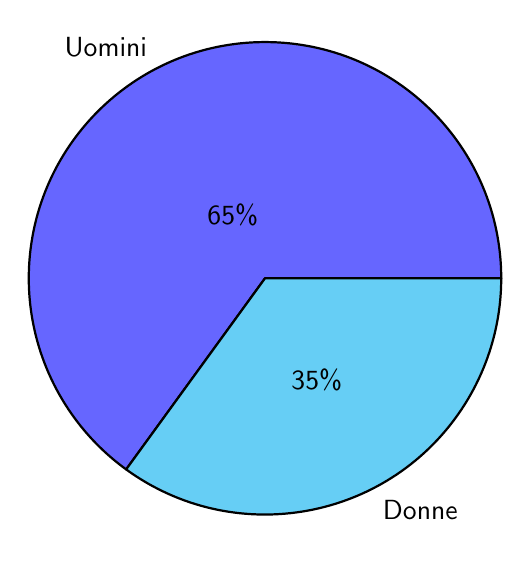
\begin{tikzpicture}
        \pie{65/Uomini, 35/Donne}
    \end{tikzpicture}
    \caption{Gender Dataset}
    \label{fig:torta}
\end{figure}

Il dataset inoltre presenta dati presi da un ambiente Americano, il che porta un cattivo adattamento generale dovuto al differente sistema scolastico e di votazione \textit{(vedi Table 1)}.

\begin{table}[ht]
    \centering
    \begin{tabular}{|c|c|}
        \hline
        Voto Americano & Voto Italiano \\
        \hline
        Grado A        & 70-110        \\
        Grado B        & 60-70         \\
        Grado C        & 50-60         \\
        ...            & ...           \\
        \hline
    \end{tabular}
    \caption{Esempio di voti}
\end{table}

\newpage

\subsection{Data Preparation}
In questa sezione, tratteremo le adottate per preparare i dati acquisiti in modo che il nostro machine learner
non dia problemi.

Il data preparation si articola nei seguenti quattro passaggi:

\begin{enumerate}
    \item \textbf{Data cleaning;}
    \item \textbf{Feature scaling;}
    \item \textbf{Feature selection;}
    \item \textbf{Data balancing;}
\end{enumerate}

\subsubsection{Data cleaning}
Il \textit{Data Cleaning}, definito come \textit{"Pulizia dei dati"}, si occupa di rimediare a problemi quando ci sono righe
di dati mancanti ma più in generale ha come obiettivo quello di fornire un dataset dotato di una qualità adeguata.
Nel nostro dataset non sono presenti dati mancanti e di conseguenza non abbiamo effettuato la fase di \textit{Data Imputation}, che
sarebbe la fase dove si stimano i valori dei dati mancanti. Oltretutto non è stato necessario effettuare una normalizzazione
sui dati.

\subsubsection{Feature scaling}

\subsubsection{Feature selection}
Il \textit{Feature selection} rientra nell'ambito del feature engeneering, che sarebbe il processo nel quale il progettista
utilizza la propria conoscenza del dominio per determinare le caratteristiche (feature) dai dati grezzi estraibile tramite tecniche
di data mining.

Nel nostro caso abbiamo pensato di rimuovere colonne che non erano adeguate per il nostro obiettivo ovvero, quello di creare
un software che preveda un piazzamento nel mondo del lavoro quanto più etico possibile e adeguato per studenti che studiano in
Italia.

\begin{table}[ht]
    \centering
    \begin{tabular}{|c|c|c|c|c|c|c|c|c|c|}
        \hline
        Gender & 10TH * & BESSC  & 12TH * & HSC EX & Subject  & UNDERGRAD & MAJORS    & WorkExp & Aptitude \\
        \hline
        M      & 67     & Others & 91     & Others & Commerce & 58        & Sci-Tech  & No      & 55       \\
        F      & 46     & Others & 49.2   & Others & Commerce & 79        & Comm-Mgmt & No      & 74,28    \\
        ...    & ...    & ...    & ...    & ...    & ...      & ...       & ...       & ...     & ...      \\
        \hline
    \end{tabular}
    \caption{Esempio di dati}
\end{table}

La prima colonna che abbiamo eliminato è quella riguardante il \textbf{Gender}, in quanto abbiamo pensato che non convenisse porre dei limiti
riguardanti il sesso di una persona visto che il dataset in considerazione presentava più istanze con soggetto maschile rispetto a quelle femminili
e che poteva portare ad un machine learner che descriminasse i vari gender.

Le successive colonne presentavano dati che non erano adeguati in modo universale rispetto tutti i tipi di studio nelle varie lingue
tra cui, in questo caso, l'Italiano. Il dataset presentava solo voti e riferimenti ai vari studi che riguardavano solo ed esclusivamente
l'ambito scolastico Americano. Oltretutto la tabella presenta la percentuale di riuscita di un test di ingresso aziendale, che nel nostro caso
abbiamo ritenuto giusto lasciare poichè solitamente nella maggior parte dei casi è presente.

\subsubsection{Data balancing}

\end{document}
